\documentclass[tikz,border=2pt]{standalone}
\usepackage{amsmath,amssymb}
\usepackage{tikz}

\begin{document}
% Naive probability: 36 equally likely outcomes for two dice; the 6 highlighted cells have
% sum 7, so P(sum = 7) = 6/36.
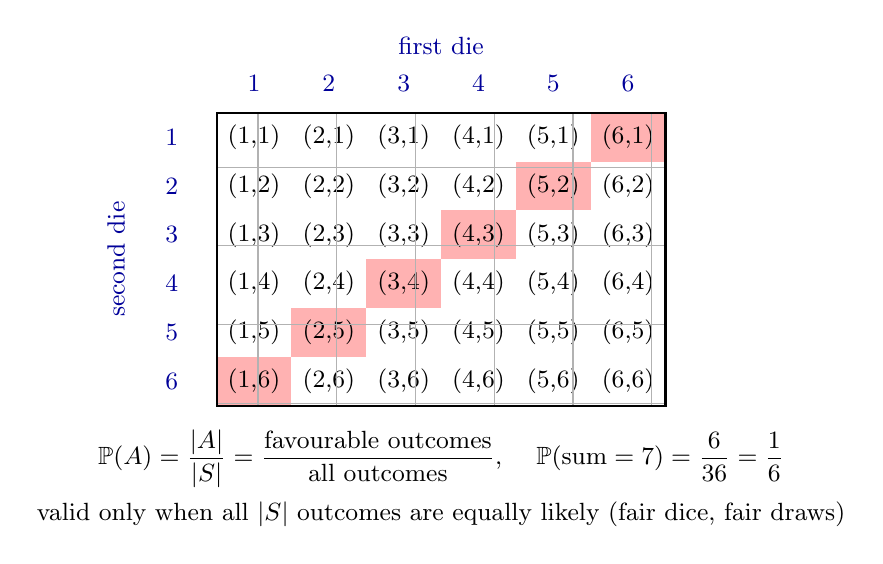
\begin{tikzpicture}[every node/.style={font=\small}, x=0.95cm, y=0.62cm]
	\foreach \i in {1,...,6} {\foreach \j in {1,...,6} {
		\pgfmathtruncatemacro{\s}{\i+\j}
		\ifnum\s=7 \fill[red!30] (\i-0.5,-\j+0.5) rectangle (\i+0.5,-\j-0.5); \fi
		\node[font=\small] at (\i,-\j) {(\i,\j)};
	}}
	\draw[gray!60] (0.5,-0.5) grid (6.5,-6.5);
	\draw[thick] (0.5,-0.5) rectangle (6.5,-6.5);
	\foreach \i in {1,...,6} {\node[font=\small, blue!60!black] at (\i,0.1) {\i}; \node[font=\small, blue!60!black] at (-0.1,-\i) {\i};}
	\node[blue!60!black, anchor=south] at (3.5,0.5) {first die};
	\node[blue!60!black, anchor=east, rotate=90] at (-0.6,-3.5) {};
	\node[blue!60!black, rotate=90, anchor=south] at (-0.6,-3.5) {second die};
	\node[anchor=north, align=center] at (3.5,-6.8) {$\mathbb{P}(A)=\dfrac{|A|}{|S|}=\dfrac{\text{favourable outcomes}}{\text{all outcomes}}$, \quad $\mathbb{P}(\text{sum}=7)=\dfrac6{36}=\dfrac16$\\[4pt] valid only when all $|S|$ outcomes are equally likely (fair dice, fair draws)};
\end{tikzpicture}
\end{document}
